\section{Neural Radiance Fields - NeRFs}
\label{NeRF}

NeRF - Acronym for Neural Radiance Fields. Neural as there a neural network. Radiance as the neural network describes the radiance of the scenes (how much light is been emitted by a point in space and in each direction). Field as this is a continuous function - a smooth thing that exists in the world. 

Neural Radiance Fields (NeRFs) \citep{mildenhallNERF} offer an alternative approach to representing 3D scenes from a limited set of 2D images, as introduced by \citeauthor{mildenhallNERF}. Unlike traditional 3D reconstruction methods, NeRFs use a volumetric representation to accurately capture both the spatial and angular distribution of light. Traditional techniques often fall short in capturing complex geometries and variable lighting conditions, issues that NeRFs successfully address by modeling the volumetric scene as a continuous 5D function. This function accepts 3D spatial coordinates and viewing direction as inputs and produces the color and opacity at a specific point in the scene.
This approach contrasts with classic deep learning methods, which require a comprehensive dataset comprising various scenes and their representations. NeRFs, however, are trained to specialize in a single, unique scene \citep{mildenhallNERF}. The neural network consists of layers specifically designed to encode the volumetric details of that particular scene, effectively creating a dedicated neural network for each scene.

\textcolor{blue}{One of the notable strengths of NeRFs lies in their capability for view-dependent appearance modeling. The system considers how the appearance of an object or scene varies with the direction from which it is viewed, offering a more nuanced and realistic visual impression. This view-dependent feature of NeRFs enables the synthesis of images that accurately reflect how differently the same scene or object can appear when viewed from different angles. In addition, NeRFs offer the ability to capture more complicated geometries and occlusions. The method is capable of producing detailed depth maps that are often difficult to obtain using traditional techniques, especially for complex scenes. These depth maps are versatile enough to support mixed reality applications and allow seamless integration of virtual objects into real-world environments. The system also facilitates the conversion of Neural Radiance Fields into 3D mesh structures using marching cubes, further increasing their usefulness. Another advantage of using NeRFs is their ability to process real-world objects captured through inward-looking 360-degree views. Unlike many other methods, NeRFs do not require background isolation or masking, making them suitable for a wide range of applications. They can synthesize any intermediate view between captured images, providing a complete and flexible representation of the object or scene.
https://www.matthewtancik.com/nerf}

\begin{figure}[ht]
    \centering
      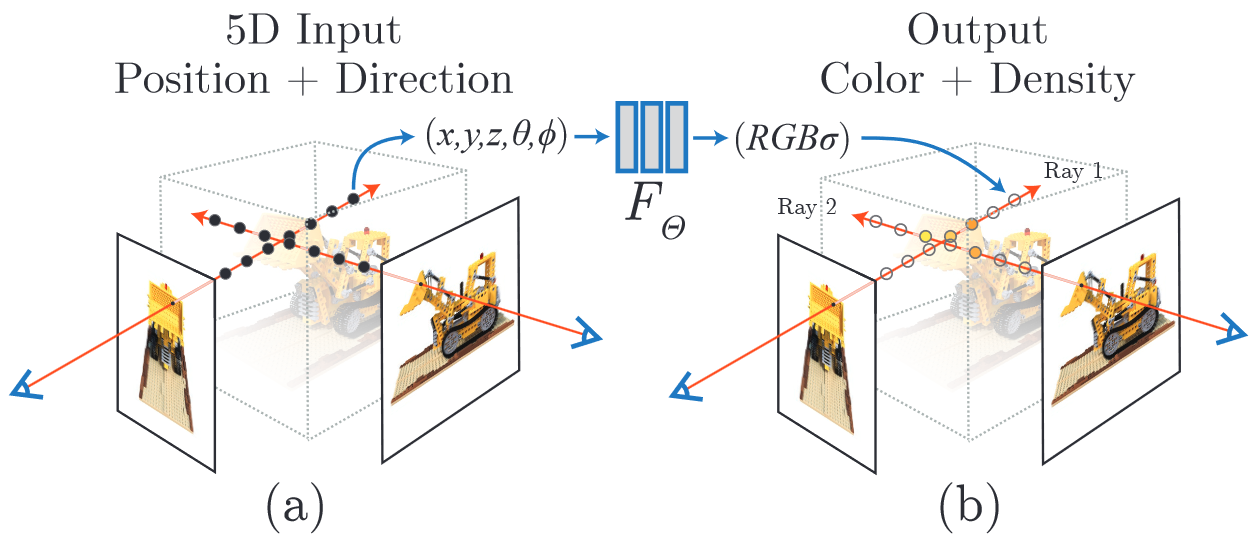
\includegraphics[width=1\columnwidth]{figures/NeRF_Fig_2_Mildenhall.png}
      \caption{Neuronal Radiance Field. Figure taken From Mildenhall \cite{mildenhallNERF} - Figure 2}
      \label{fig:figureNeRF}
\end{figure}

The neural network accepts two types of input: a position in a given coordinate system, often expressed as a 3D vector \(x, y, z\), and a viewing direction \(d\). The network's output consists of the color \(c\) and density \( \sigma \) at that particular location \citep{mildenhallNERF}. Queries to the neural network can be made by projecting a ray through the scene and asking for color and density information at various points along the ray. This enables capturing complex visual phenomena like lighting, reflections, and transparency. 
For each pixel in a desired image frame, a similar querying process is performed. The neural network is queried at multiple points along a ray projected through the scene to produce a curve representing the density of objects along the ray's path, as seen in part (c) of Figure \ref{fig:figureNeRF}. The point at which this density curve rises ignificantly usually corresponds to an object in the scene, and the color at this point is what is rendered for that particular pixel. These density and color curves can be visualized using graphs to illustrate how density and color vary along the ray's path. For instance, if a ray intersects a tree, the density would increase and the color output would likely be green, representing the tree's leaves. 
The network can also handle multi-view consistency, predicting color as a function of both location and viewing direction, while density is predicted solely based on location. The idea is that density, or transparency, is invariant to the direction from which an object is viewed. Therefore, to generate the color, the model first computes the density and a hidden representation based on the location. This hidden representation is then concatenated with the viewing direction and passed through another set of layers to produce the color.

An integral aspect of setting up NeRFs involves solving the problem of identifying the camera's position and direction for each input image. Methods like structure-from-motion and SLAM can address this issue. Once these are identified, new views can be synthesized by querying the neural network for color and density information along rays projected through the scene. 
Another challenge arises during training due to the absence of explicit density information. Nevertheless, the training process can be managed by minimizing the loss between predicted and observed values from input images. The model employs backpropagation, as its entire pipeline for rendering images, which includes casting rays, sampling alone these rays, and integrating the sampled values to compute a pixel's color, is differentiable.

In Neural Radiance Fields (NeRF), volume rendering with radiance fields utilizes the formula \[ C(r) = \int_{t_n}^{t_f} T(t)\sigma(r(t))c(r(t), d)dt \], where \[ T(t) = \exp\left(-\int_{t_n}^t \sigma(r(s))ds\right) \] This formula allows for the rendering of a 3D scene by casting rays and integrating their properties from a near boundary to a far boundary. Specifically, \( T(t) \) represents the probability of a ray passing through empty space up to a certain point, influenced by the density function \( \sigma \). This calculation determines whether the ray continues through empty space or ends when it hits an object, with color adjustments made at this endpoint. The model can also capture complex details such as transparency. Although Naive NeRF models cannot provide photorealistic results due to the lack of detail, several optimizations have been introduced to improve their performance. One of these improvements is the use of position encoding techniques that deterministically map 3D coordinates and view directions to a higher dimensional space using a hierarchical series of sine and cosine functions. This approach differs from position coding in transformer models and is used to capture both fine and coarse detail in 3D space. Another optimization involves hierarchical volume sampling by a two-level neural network system consisting of "coarse" and "fine" layers. The coarse network initially sparsely samples the rays in the 3D scene and provides instructions to the fine network for more detailed sampling. While both meshes are optimized simultaneously, the final rendering is based solely on the fine mesh.

The experimental results indicate several key strengths and limitations of the Neural Radiance Fields (NeRF) approach. One of its notable advantages is the model's ability to handle fine-grained structures, which is particularly evident when examining the details of rendered objects like a microphone. Another significant benefit is the model's efficiency in terms of memory usage. For example, a single scene rendered using NeRF only occupies about five megabytes of memory, a stark contrast to voxel grid representations that can consume over 15 gigabytes for the same scene. Intriguingly, the memory footprint of the rendered scene is even smaller than that of the input images, making the model highly efficient for data storage and transmission. However, the model is not without drawbacks. One limitation is the computational cost involved in training the neural network. The optimization process for a single scene can require around 100,000 to 300,000 iterations to converge when using a single NVIDIA V100 GPU, translating to a training time of approximately one to two days. Although this doesn't necessitate a data center, it does require a significant amount of time. The authors also conducted ablation studies to understand the contributions of various model components. The results underscore the importance of positional encodings and view-dependent effects. Omitting positional encodings or view dependence negatively impacts the model's ability to capture realistic light effects and fine-grained structures, respectively. Therefore, these components are crucial for the model's performance and its ability to render scenes with high fidelity.

- Limited rendering model: difficult to optimize
+ Highly compressible (1-10MB)